\documentclass[]{elsarticle} %review=doublespace preprint=single 5p=2 column
%%% Begin My package additions %%%%%%%%%%%%%%%%%%%
\usepackage[hyphens]{url}

  \journal{Journal of Human Evolution} % Sets Journal name


\usepackage{lineno} % add
  \linenumbers % turns line numbering on
\providecommand{\tightlist}{%
  \setlength{\itemsep}{0pt}\setlength{\parskip}{0pt}}

\usepackage{graphicx}
\usepackage{booktabs} % book-quality tables
%%%%%%%%%%%%%%%% end my additions to header

\usepackage[T1]{fontenc}
\usepackage{lmodern}
\usepackage{amssymb,amsmath}
\usepackage{ifxetex,ifluatex}
\usepackage{fixltx2e} % provides \textsubscript
% use upquote if available, for straight quotes in verbatim environments
\IfFileExists{upquote.sty}{\usepackage{upquote}}{}
\ifnum 0\ifxetex 1\fi\ifluatex 1\fi=0 % if pdftex
  \usepackage[utf8]{inputenc}
\else % if luatex or xelatex
  \usepackage{fontspec}
  \ifxetex
    \usepackage{xltxtra,xunicode}
  \fi
  \defaultfontfeatures{Mapping=tex-text,Scale=MatchLowercase}
  \newcommand{\euro}{€}
\fi
% use microtype if available
\IfFileExists{microtype.sty}{\usepackage{microtype}}{}
\bibliographystyle{elsarticle-harv}
\usepackage{longtable}
\usepackage{graphicx}
% We will generate all images so they have a width \maxwidth. This means
% that they will get their normal width if they fit onto the page, but
% are scaled down if they would overflow the margins.
\makeatletter
\def\maxwidth{\ifdim\Gin@nat@width>\linewidth\linewidth
\else\Gin@nat@width\fi}
\makeatother
\let\Oldincludegraphics\includegraphics
\renewcommand{\includegraphics}[1]{\Oldincludegraphics[width=\maxwidth]{#1}}
\ifxetex
  \usepackage[setpagesize=false, % page size defined by xetex
              unicode=false, % unicode breaks when used with xetex
              xetex]{hyperref}
\else
  \usepackage[unicode=true]{hyperref}
\fi
\hypersetup{breaklinks=true,
            bookmarks=true,
            pdfauthor={},
            pdftitle={Ecological perspectives on technological diversity at Kanjera South},
            colorlinks=false,
            urlcolor=blue,
            linkcolor=magenta,
            pdfborder={0 0 0}}
\urlstyle{same}  % don't use monospace font for urls

\setcounter{secnumdepth}{0}
% Pandoc toggle for numbering sections (defaults to be off)
\setcounter{secnumdepth}{0}


% Pandoc header



\begin{document}
\begin{frontmatter}

  \title{Ecological perspectives on technological diversity at Kanjera South}
      
  \begin{abstract}
  The aspects of hominin behavior responsible for Oldowan stone tool
  variation are the focus of much debate. There is some consensus that
  Oldowan artifact variation arises from a combination of ecological and
  cultural factors. These factors are often examined independently of one
  another. The diversity of raw material types and technological
  strategies present at Kanjera South, Kenya provide an opportunity to
  examine the interaction of ecology and culture on Oldowan stone tool
  variation. Here we combine previous analyses of raw material properties,
  provenance, and technology with quantitative measures of core reduction
  intensity and tool utilization to examine the influence of both
  ecological and techno-cultural factors on stone tool variation at
  Kanjera South. The results of this analysis reflect a dynamic
  relationship between raw material properties, provenance, and hominin
  mobility. Exotic raw materials are generally more resistant to edge
  attrition compared to those available locally, which may have
  incentivized their transport over long distances and more extensive
  reduction. Cores produced on raw materials from distant sources also
  exhibit more complex core reduction strategies than locally acquired
  materials. While this pattern is partially due to the differences in the
  quality of knappable stone, bifacial centripetal and multifacial core
  reduction strategies also arise due to the continuous transport and use
  of exotic raw materials. Moreover, the variation in stone tool reduction
  is not consistent with neutral models of stone tool transport and
  discard. These results demonstrate that ecological factors such as raw
  material provenance and physical properties have strong impacts on
  reduction intensity and the technological strategies utilized by
  hominins. Oldowan stone tool variation should not be examined from a
  strictly ecological or technological perspective, but rather within the
  context of its broader cultural-ecological system.
  \end{abstract}
  
 \end{frontmatter}

\hypertarget{introduction}{%
\section{1.0 Introduction}\label{introduction}}

Upon its initial discovery, the Oldowan was considered an expedient
industry that was akin to simply smashing stones. Nearly a century
later, the Oldowan is now known to reflect a complex behavioral pattern
that encompasses not only the technical capacity to efficiently produce
flakes, but also dynamic patterns of transport. Technological analyses
show that Oldowan hominins had at least a basic understanding of the
general principles of flaking and selection of suitable tool stones for
artifact manufacture (Semaw, 2000; de la Torre, 2004; Delagnes and
Roche, 2005; Stout et al., 2005; Schick et al., 2006; Braun et al.,
2009b, 2019; Goldman-Neuman and Hovers, 2012). This pattern of tool
production was integrated into a broader land-use strategy in which raw
material is acquired, transported, utilized, maintained and eventually
discarded (Hay, 1976; Isaac and Harris, 1976; Isaac, 1981, 1984; Toth,
1985, 1987; Schick, 1987; Potts, 1991, 1994; Blumenschine and Peters,
1998; Potts et al., 1999; Blumenschine et al., 2008; Braun et al.,
2008a). Though these actions remained simple, the various ways in which
they are combined create a variety of production strategies that can be
evaluated on a site-by-site basis (Delagnes and Roche, 2005).

Research on these topics has revealed a multitude of technological
diversity in the Oldowan across time and space. A primary objective of
current Oldowan research is identifying the behavioral processes in
which such a diversity of production strategies arise (Plummer, 2004;
Roche et al., 2009; Gallotti, 2018). A multitude of work now links the
technical diversity of the Oldowan to the cognition, skill, the social
transmission of information, and, in some cases, the social learning
mechanisms of Plio-Pleistocene hominins (Schick and Toth, 1994; Hovers,
2009, 2012; Stout and Chaminade, 2009; Stout, 2011; Goldman-Neuman and
Hovers, 2012; Roche et al., 2018; Toth and Schick, 2018; Stout et al.,
2019). However, while our understanding of technical decision making has
dramatically increased, research focusing on ecological influences on
Oldowan technological diversity, such as land-use and tool transport,
has waned in recent decades (de Torre and Mora, 2009).

Though stone tool diversity is linked to constraints imposed by raw
material geometry, quality, and abundance (Toth, 1982, 1985, 1987;
Potts, 1988, 1991; de la Torre, 2004; Blumenschine et al., 2008; Braun
et al., 2009a), how hominin tool transport and more broadly land-use
patterns influence the technical decision making of Oldowan tool makers
remains unclear. Early work on this subject has suggested that the
technological diversity in the Oldowan points to a continuum of
reduction as stone is moved across the landscape (Toth, 1985; Potts,
1991). While Potts (1991) illustrated an interesting relationship
between mass and Leakey's typological core categories, little work has
been done to further establish connections between hominin land-use and
technological diversity. With the advent of new quantitative methods and
our much-expanded knowledge of the Oldowan, further investigation into
this pattern would enhance our understanding of Oldowan technical
decision making, land use, and the stone tool variation in the Oldowan.

The \textasciitilde{}2.0 ma site of Kanjera South contributes to our
understanding of the relationship between stone tool production,
technical decision making and hominin behavioral ecology. The lithic
assemblage at Kanjera South shows a substantial representation of exotic
raw materials (e.g.~rock types not available within 10 km of the
archaeological site) and a diversity of different core reduction
strategies that, when combined with novel statistical analyses, provide
an opportunity to understand the technical decision making within the
context of broader hominin land-use strategies. Although early Oldowan
assemblages dating to 2.0 million years ago and older illustrate a
similar level of technological competence to those from later
timeframes, substantially less is known about the broader foraging
behaviors and land-use strategies of hominins during this interval. An
investigation of hominin stone tool transport and utilization patterns
at Kanjera would not only add to our understanding of how the landscape
structures stone tool-use and transport but also further elucidate the
relationship between Oldowan technological strategies and the land-use
patterns.

To this end, we present a novel study of the Kanjera South lithic
material that combines previous analyses of raw material properties,
provenance, and technology with quantitative measures of core reduction
intensity and tool utilization to elucidate the broader land-use
pattern. In doing so, we show that the technological variation at
Kanjera South reflects an interaction of raw material properties,
foraging ecology, and landscape scale constraints on raw material
availability. Not only are we able to characterize the broader pattern
of land-use of Oldowan hominins at Kanjera South, but we also show that
this pattern may condition the economization of stone resources across
space. This study not only sheds light on the environmental and
technical variables that contribute to Oldowan stone tool variability,
but also provides a unique insight into hominin land-use patterns during
the early part of the Oldowan industry.

\hypertarget{background-to-kanjera-south}{%
\section{2.0 Background to Kanjera
South}\label{background-to-kanjera-south}}

The \textasciitilde{}2.0 Ma site of Kanjera South is situated on the
northeastern side of the Homa Peninsula on the edges of the Nyanza Rift
near the shores of Lake Victoria (Plummer et al., 1999; Ditchfield et
al., 2019, Fig. \ref{map}). The extensive excavation of a 3 meter deep
sequence of silts and clays recovered over 3000 fossils and similar
numbers of stone artifacts (Plummer et al., 2009a). The stratigraphy at
Kanjera South is made up of approximately 30 meters of fluvial,
colluvial and lacustrine sediments (Ditchfield et al., 2019). Extensive
research on the geochronology and sedimentary context has demonstrated
that the lithics and fossils accumulated predominantly by hominin
activity (Behrensmeyer et al., 1995; Plummer et al., 2009a, 2009b;
Ferraro et al., 2013; Ditchfield et al., 2019). The frequencies of
different bovids and enamel isotope studies indicate that the landscape
surrounding Kanjera South, unlike the setting of many Oldowan sites, was
dominated by a grassland as opposed to more closed habitats (Plummer et
al., 2009b, 2009a). Zooarchaeological evidence at Kanjera South strongly
implicates a scenario where hominins had early access to small carcasses
and mixed access to larger carcasses (Oliver et al., 2019). This record
is consistent through the stratified sequence, suggesting that
persistent carnivory spanned hundreds to thousands of years (Ferraro et
al., 2013). Though Kanjera South is considered to have been of
significance to hominins, it is difficult to determine if there was
something unique about its location specifically or if the Homa
Pennisula as a whole, was simply a hospitable place (Behrensmeyer et
al., 1995). Substantial faulting in the region makes it difficult to
assess the ecological qualities of Kanjera South within a broader
landscape context.

\begin{figure}
\centering
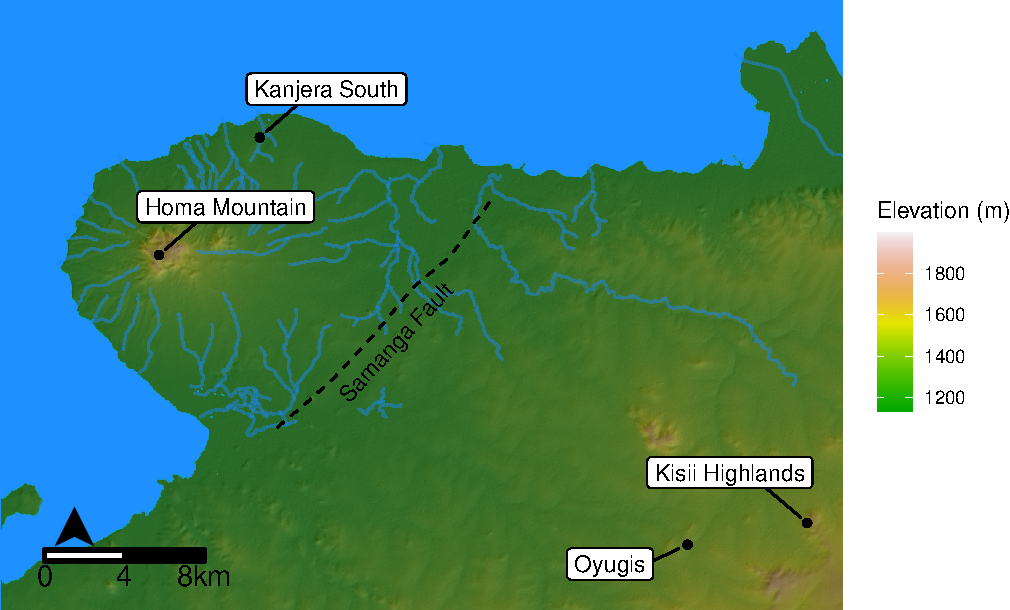
\includegraphics{HUMEV-D-20-00115_revised_draft_files/figure-latex/fig-1-1.pdf}
\caption{A map of the Homa Peninsula. Kanjera South is situated to the
East of Homa Mountain. The Homa Mountain carbonatite center is the
primary source of the local raw materials including Homa limestone
(HLi), Homa Phonolite (HPh), and Fenetized nyanzian rocks (FNy).
Drainages coming off the flanks of Homa Mountain carry these local rock
types to within the immediate vicinity of Kanjera South. Distant or
exotic raw materials originate in river conglomerates much farther to
the east of the Samanga Fault. These include Bukoban andesite (BBa),
Bukoban felsite (BFe), Bukoban quartzite (BQu), Nyanzian rhyolite (NyR),
and Oyugis granite (OGr) \label{map}}
\end{figure}

Extensive geological surveys of the Homa Peninsula and the surrounding
area reveal a high diversity of igneous and metamorphic rocks that
provided a wide range of suitable materials that hominins could utilize
for flake production (Saggerson, 1952; Le Bas, 1977; Braun et al.,
2008a; Finestone et al., 2020). As such, this diversity is reflected in
the lithic assemblage. More than 16 different rock types are represented
in the assemblage although the bulk of the material is produced on 8 of
them (Braun et al., 2008a). Geochemical provenance studies of the lithic
material make it possible to further subdivide the lithic assemblage to
two broad categories: local and exotic (Table \ref{table1}; Braun et
al., 2008a). Local materials are derived from the Homa Mountain
Carbonatite center (Fig. \ref{map}). Drainages running off the flanks of
this mountain would have carried materials such as phonolite, limestone,
and fenetized rocks within the immediate vicinity of Kanjera South.
Sources of the exotic materials, such as quartzite, rhyolite, andesite,
and granite are located further to the east in places such as the Kisi
Highlands and Oyugis (Fig. \ref{map}). While these materials were likely
acquired from river channels traveling west-ward toward Kanjera South,
they are not present in Pleistocene river conglomerates within 10
kilometers of Kanjera South (Braun et al., 2008a).

\begin{longtable}[]{@{}llll@{}}
\caption{A list of rock types found at Kanjera South included in this
analysis \label{table1}}\tabularnewline
\toprule
Raw Material & Abreviation & Origin & Provenance\tabularnewline
\midrule
\endfirsthead
\toprule
Raw Material & Abreviation & Origin & Provenance\tabularnewline
\midrule
\endhead
Fenetized nyanzian & FNy & Homa Mountain & Local\tabularnewline
Homa limestone & HLi & Homa Mountain & Local\tabularnewline
Homa phonolite & HPh & Homa Mountain & Local\tabularnewline
Bukoban andesite & BBa & East of Samanga Fault & Exotic\tabularnewline
Bukoban felsite & BFe & East of Samanga Fault & Exotic\tabularnewline
Bukoban quartzite & BQu & East of Samanga Fault & Exotic\tabularnewline
Nyanzian rhyolite & NyR & East of Samanga Fault & Exotic\tabularnewline
Oyugis granite & OGr & Oyugis & Exotic\tabularnewline
\bottomrule
\end{longtable}

The Kanjera South lithic assemblage is distinguished from other Oldowan
assemblages by the number of raw materials represented, as well as the
diversity of technological production strategies present within the
assemblage. Unlike most other Oldowan sites from this timeframe which
have a predominate core reduction strategy present (see Gallotti, 2018),
the flake production strategies at Kanjera South range from simple
unifacial techniques to bifacial and multifacial techniques (Fig.
\ref{tools}). Previous work has suggested that some of this diversity
reflects the differences in the quality of available raw materials or
the need to maximize the amount of flakes removed from high quality
materials (Braun et al., 2009a). The wide range in diversity of
materials from local and exotic sources, and technological reduction
strategies, provide an opportunity to investigate the dynamics between
hominin land-use patterns, stone tool production, and Oldowan assemblage
variability.

\begin{figure}
\centering
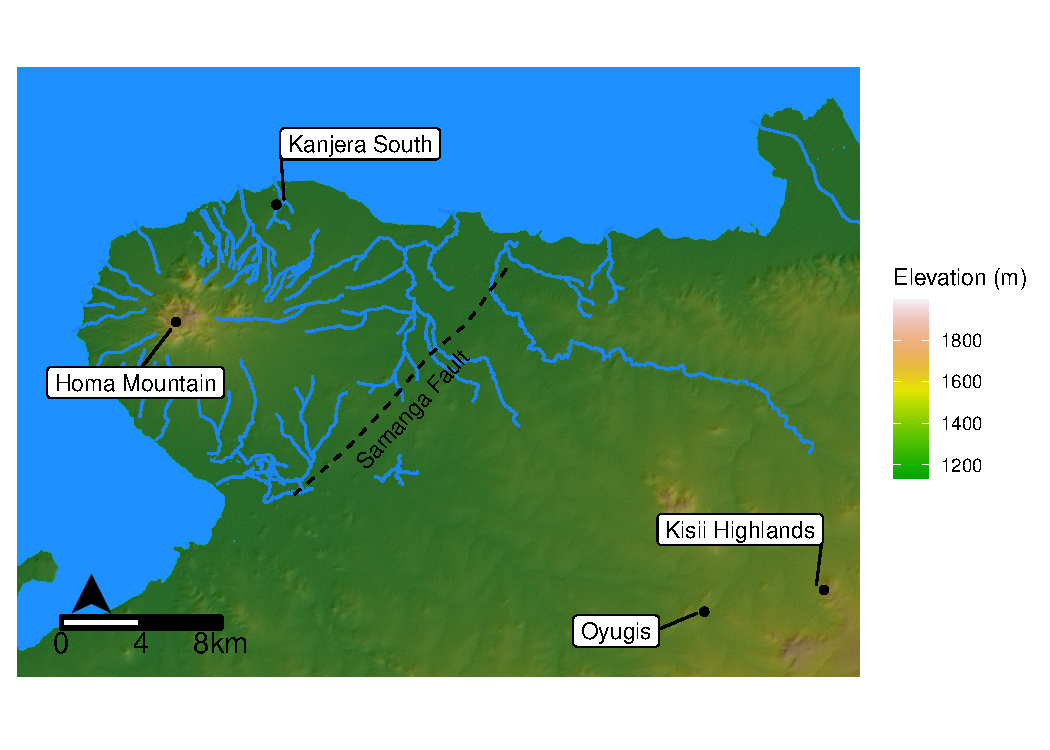
\includegraphics{HUMEV-D-20-00115_revised_draft_files/figure-latex/fig-2-1.pdf}
\caption{Examples of the stone artifacts found at Kanjera South. (A)
Core produced on Homa limestone. (B) Core produced on Oyugis granite.
(C) Core produced on Bukoban quartzite. (D) Core produced on Fenetized
nyanzian. \label{tools}}
\end{figure}

\hypertarget{materials-and-methods}{%
\section{2.0 Materials and methods}\label{materials-and-methods}}

\hypertarget{materials}{%
\subsection{2.1 Materials}\label{materials}}

To explore the relationship between stone tool transport and Oldowan
assemblage variability, we characterize the technology of stone tools
produced on both exotic and local materials at Kanjera South (Table
\ref{table1}) through the study of the core and complete flake
assemblages (i.e., our analysis at this time does not incorporate
angular fragments) (Tables \ref{table2} and \ref{table3}). Preexisting
knowledge regarding raw material provenance, raw material properties,
and core exploitation strategies (Braun et al., 2009a, 2009a, 2009b;
Finestone et al., 2020) was combined with an in-depth analysis of the
lithic material designed to quantify the intensity of stone tool
utilization prior to their discard at Kanjera South.

A total of 1500 stone artifacts (171 cores and 1329 flakes) were
analyzed using a series of continuous and ordinal variables (see below).
Tables 2 and 3 provides a detailed summary of the number of lithics per
raw material included. The raw data for this analysis can also be
accessed by following this
\href{https://www.dropbox.com/home/Models_and_Runs/Kanjera\%20South}{Link}.
In addition to the previously published technological analysis, the
cores were also categorized using de la Torre and Mora's (2005)
idealized schemes of free-hand core reduction (de la Torre Ignacio,
2011). These measurements provided a means by which to characterize the
assemblage in terms of core and flake utilization using measures of core
reduction intensity, flake sequence and edge to mass ratios.

\begin{longtable}[]{@{}lrrrrrrrrrrr@{}}
\caption{A summary of the cores included in this analysis
\label{table2}}\tabularnewline
\toprule
\begin{minipage}[b]{0.02\columnwidth}\raggedright
RM\strut
\end{minipage} & \begin{minipage}[b]{0.01\columnwidth}\raggedleft
N\strut
\end{minipage} & \begin{minipage}[b]{0.05\columnwidth}\raggedleft
Avg. Length\strut
\end{minipage} & \begin{minipage}[b]{0.04\columnwidth}\raggedleft
Avg. Width\strut
\end{minipage} & \begin{minipage}[b]{0.04\columnwidth}\raggedleft
Avg. Thick\strut
\end{minipage} & \begin{minipage}[b]{0.05\columnwidth}\raggedleft
Avg. Mass (g)\strut
\end{minipage} & \begin{minipage}[b]{0.07\columnwidth}\raggedleft
Avg. N flake scars\strut
\end{minipage} & \begin{minipage}[b]{0.11\columnwidth}\raggedleft
Avg. Exploitation Surfaces\strut
\end{minipage} & \begin{minipage}[b]{0.10\columnwidth}\raggedleft
Avg. Surface Interactions\strut
\end{minipage} & \begin{minipage}[b]{0.07\columnwidth}\raggedleft
Min. \% Mass Lost\strut
\end{minipage} & \begin{minipage}[b]{0.07\columnwidth}\raggedleft
Avg. \% Mass Lost\strut
\end{minipage} & \begin{minipage}[b]{0.07\columnwidth}\raggedleft
Max. \% Mass Lost\strut
\end{minipage}\tabularnewline
\midrule
\endfirsthead
\toprule
\begin{minipage}[b]{0.02\columnwidth}\raggedright
RM\strut
\end{minipage} & \begin{minipage}[b]{0.01\columnwidth}\raggedleft
N\strut
\end{minipage} & \begin{minipage}[b]{0.05\columnwidth}\raggedleft
Avg. Length\strut
\end{minipage} & \begin{minipage}[b]{0.04\columnwidth}\raggedleft
Avg. Width\strut
\end{minipage} & \begin{minipage}[b]{0.04\columnwidth}\raggedleft
Avg. Thick\strut
\end{minipage} & \begin{minipage}[b]{0.05\columnwidth}\raggedleft
Avg. Mass (g)\strut
\end{minipage} & \begin{minipage}[b]{0.07\columnwidth}\raggedleft
Avg. N flake scars\strut
\end{minipage} & \begin{minipage}[b]{0.11\columnwidth}\raggedleft
Avg. Exploitation Surfaces\strut
\end{minipage} & \begin{minipage}[b]{0.10\columnwidth}\raggedleft
Avg. Surface Interactions\strut
\end{minipage} & \begin{minipage}[b]{0.07\columnwidth}\raggedleft
Min. \% Mass Lost\strut
\end{minipage} & \begin{minipage}[b]{0.07\columnwidth}\raggedleft
Avg. \% Mass Lost\strut
\end{minipage} & \begin{minipage}[b]{0.07\columnwidth}\raggedleft
Max. \% Mass Lost\strut
\end{minipage}\tabularnewline
\midrule
\endhead
\begin{minipage}[t]{0.02\columnwidth}\raggedright
BBA\strut
\end{minipage} & \begin{minipage}[t]{0.01\columnwidth}\raggedleft
4\strut
\end{minipage} & \begin{minipage}[t]{0.05\columnwidth}\raggedleft
65.82\strut
\end{minipage} & \begin{minipage}[t]{0.04\columnwidth}\raggedleft
54.38\strut
\end{minipage} & \begin{minipage}[t]{0.04\columnwidth}\raggedleft
38.28\strut
\end{minipage} & \begin{minipage}[t]{0.05\columnwidth}\raggedleft
198.380\strut
\end{minipage} & \begin{minipage}[t]{0.07\columnwidth}\raggedleft
8\strut
\end{minipage} & \begin{minipage}[t]{0.11\columnwidth}\raggedleft
2\strut
\end{minipage} & \begin{minipage}[t]{0.10\columnwidth}\raggedleft
2\strut
\end{minipage} & \begin{minipage}[t]{0.07\columnwidth}\raggedleft
11\strut
\end{minipage} & \begin{minipage}[t]{0.07\columnwidth}\raggedleft
66\strut
\end{minipage} & \begin{minipage}[t]{0.07\columnwidth}\raggedleft
89\strut
\end{minipage}\tabularnewline
\begin{minipage}[t]{0.02\columnwidth}\raggedright
BFE\strut
\end{minipage} & \begin{minipage}[t]{0.01\columnwidth}\raggedleft
15\strut
\end{minipage} & \begin{minipage}[t]{0.05\columnwidth}\raggedleft
60.87\strut
\end{minipage} & \begin{minipage}[t]{0.04\columnwidth}\raggedleft
47.02\strut
\end{minipage} & \begin{minipage}[t]{0.04\columnwidth}\raggedleft
35.28\strut
\end{minipage} & \begin{minipage}[t]{0.05\columnwidth}\raggedleft
137.447\strut
\end{minipage} & \begin{minipage}[t]{0.07\columnwidth}\raggedleft
6\strut
\end{minipage} & \begin{minipage}[t]{0.11\columnwidth}\raggedleft
3\strut
\end{minipage} & \begin{minipage}[t]{0.10\columnwidth}\raggedleft
2\strut
\end{minipage} & \begin{minipage}[t]{0.07\columnwidth}\raggedleft
29\strut
\end{minipage} & \begin{minipage}[t]{0.07\columnwidth}\raggedleft
58\strut
\end{minipage} & \begin{minipage}[t]{0.07\columnwidth}\raggedleft
95\strut
\end{minipage}\tabularnewline
\begin{minipage}[t]{0.02\columnwidth}\raggedright
BQU\strut
\end{minipage} & \begin{minipage}[t]{0.01\columnwidth}\raggedleft
19\strut
\end{minipage} & \begin{minipage}[t]{0.05\columnwidth}\raggedleft
47.30\strut
\end{minipage} & \begin{minipage}[t]{0.04\columnwidth}\raggedleft
36.31\strut
\end{minipage} & \begin{minipage}[t]{0.04\columnwidth}\raggedleft
25.51\strut
\end{minipage} & \begin{minipage}[t]{0.05\columnwidth}\raggedleft
51.932\strut
\end{minipage} & \begin{minipage}[t]{0.07\columnwidth}\raggedleft
8\strut
\end{minipage} & \begin{minipage}[t]{0.11\columnwidth}\raggedleft
3\strut
\end{minipage} & \begin{minipage}[t]{0.10\columnwidth}\raggedleft
3\strut
\end{minipage} & \begin{minipage}[t]{0.07\columnwidth}\raggedleft
44\strut
\end{minipage} & \begin{minipage}[t]{0.07\columnwidth}\raggedleft
74\strut
\end{minipage} & \begin{minipage}[t]{0.07\columnwidth}\raggedleft
94\strut
\end{minipage}\tabularnewline
\begin{minipage}[t]{0.02\columnwidth}\raggedright
NYR\strut
\end{minipage} & \begin{minipage}[t]{0.01\columnwidth}\raggedleft
19\strut
\end{minipage} & \begin{minipage}[t]{0.05\columnwidth}\raggedleft
50.38\strut
\end{minipage} & \begin{minipage}[t]{0.04\columnwidth}\raggedleft
36.61\strut
\end{minipage} & \begin{minipage}[t]{0.04\columnwidth}\raggedleft
23.89\strut
\end{minipage} & \begin{minipage}[t]{0.05\columnwidth}\raggedleft
50.987\strut
\end{minipage} & \begin{minipage}[t]{0.07\columnwidth}\raggedleft
7\strut
\end{minipage} & \begin{minipage}[t]{0.11\columnwidth}\raggedleft
3\strut
\end{minipage} & \begin{minipage}[t]{0.10\columnwidth}\raggedleft
2\strut
\end{minipage} & \begin{minipage}[t]{0.07\columnwidth}\raggedleft
19\strut
\end{minipage} & \begin{minipage}[t]{0.07\columnwidth}\raggedleft
61\strut
\end{minipage} & \begin{minipage}[t]{0.07\columnwidth}\raggedleft
95\strut
\end{minipage}\tabularnewline
\begin{minipage}[t]{0.02\columnwidth}\raggedright
OGR\strut
\end{minipage} & \begin{minipage}[t]{0.01\columnwidth}\raggedleft
16\strut
\end{minipage} & \begin{minipage}[t]{0.05\columnwidth}\raggedleft
68.43\strut
\end{minipage} & \begin{minipage}[t]{0.04\columnwidth}\raggedleft
59.52\strut
\end{minipage} & \begin{minipage}[t]{0.04\columnwidth}\raggedleft
43.13\strut
\end{minipage} & \begin{minipage}[t]{0.05\columnwidth}\raggedleft
276.371\strut
\end{minipage} & \begin{minipage}[t]{0.07\columnwidth}\raggedleft
9\strut
\end{minipage} & \begin{minipage}[t]{0.11\columnwidth}\raggedleft
3\strut
\end{minipage} & \begin{minipage}[t]{0.10\columnwidth}\raggedleft
2\strut
\end{minipage} & \begin{minipage}[t]{0.07\columnwidth}\raggedleft
31\strut
\end{minipage} & \begin{minipage}[t]{0.07\columnwidth}\raggedleft
59\strut
\end{minipage} & \begin{minipage}[t]{0.07\columnwidth}\raggedleft
86\strut
\end{minipage}\tabularnewline
\begin{minipage}[t]{0.02\columnwidth}\raggedright
HLI\strut
\end{minipage} & \begin{minipage}[t]{0.01\columnwidth}\raggedleft
13\strut
\end{minipage} & \begin{minipage}[t]{0.05\columnwidth}\raggedleft
54.53\strut
\end{minipage} & \begin{minipage}[t]{0.04\columnwidth}\raggedleft
42.21\strut
\end{minipage} & \begin{minipage}[t]{0.04\columnwidth}\raggedleft
28.01\strut
\end{minipage} & \begin{minipage}[t]{0.05\columnwidth}\raggedleft
86.873\strut
\end{minipage} & \begin{minipage}[t]{0.07\columnwidth}\raggedleft
4\strut
\end{minipage} & \begin{minipage}[t]{0.11\columnwidth}\raggedleft
3\strut
\end{minipage} & \begin{minipage}[t]{0.10\columnwidth}\raggedleft
2\strut
\end{minipage} & \begin{minipage}[t]{0.07\columnwidth}\raggedleft
17\strut
\end{minipage} & \begin{minipage}[t]{0.07\columnwidth}\raggedleft
41\strut
\end{minipage} & \begin{minipage}[t]{0.07\columnwidth}\raggedleft
69\strut
\end{minipage}\tabularnewline
\begin{minipage}[t]{0.02\columnwidth}\raggedright
HPH\strut
\end{minipage} & \begin{minipage}[t]{0.01\columnwidth}\raggedleft
42\strut
\end{minipage} & \begin{minipage}[t]{0.05\columnwidth}\raggedleft
58.81\strut
\end{minipage} & \begin{minipage}[t]{0.04\columnwidth}\raggedleft
42.63\strut
\end{minipage} & \begin{minipage}[t]{0.04\columnwidth}\raggedleft
28.60\strut
\end{minipage} & \begin{minipage}[t]{0.05\columnwidth}\raggedleft
79.777\strut
\end{minipage} & \begin{minipage}[t]{0.07\columnwidth}\raggedleft
4\strut
\end{minipage} & \begin{minipage}[t]{0.11\columnwidth}\raggedleft
2\strut
\end{minipage} & \begin{minipage}[t]{0.10\columnwidth}\raggedleft
1\strut
\end{minipage} & \begin{minipage}[t]{0.07\columnwidth}\raggedleft
14\strut
\end{minipage} & \begin{minipage}[t]{0.07\columnwidth}\raggedleft
40\strut
\end{minipage} & \begin{minipage}[t]{0.07\columnwidth}\raggedleft
84\strut
\end{minipage}\tabularnewline
\begin{minipage}[t]{0.02\columnwidth}\raggedright
FNY\strut
\end{minipage} & \begin{minipage}[t]{0.01\columnwidth}\raggedleft
38\strut
\end{minipage} & \begin{minipage}[t]{0.05\columnwidth}\raggedleft
53.29\strut
\end{minipage} & \begin{minipage}[t]{0.04\columnwidth}\raggedleft
38.52\strut
\end{minipage} & \begin{minipage}[t]{0.04\columnwidth}\raggedleft
22.77\strut
\end{minipage} & \begin{minipage}[t]{0.05\columnwidth}\raggedleft
63.947\strut
\end{minipage} & \begin{minipage}[t]{0.07\columnwidth}\raggedleft
4\strut
\end{minipage} & \begin{minipage}[t]{0.11\columnwidth}\raggedleft
2\strut
\end{minipage} & \begin{minipage}[t]{0.10\columnwidth}\raggedleft
1\strut
\end{minipage} & \begin{minipage}[t]{0.07\columnwidth}\raggedleft
7\strut
\end{minipage} & \begin{minipage}[t]{0.07\columnwidth}\raggedleft
33\strut
\end{minipage} & \begin{minipage}[t]{0.07\columnwidth}\raggedleft
72\strut
\end{minipage}\tabularnewline
\bottomrule
\end{longtable}

\hypertarget{estimating-core-reduction-intensity}{%
\subsection{2.2 Estimating Core Reduction
Intensity}\label{estimating-core-reduction-intensity}}

The reduction intensity of cores influences a variety of attributes that
interact throughout the reduction sequence (Douglass et al., 2018). As a
result, core reduction intensity is understood from a diversity of
variables ranging from mass, the number of flake scars, to more
sophisticated methods that use linear models to estimate the degree to
which a core has been reduced (Toth, 1985; Potts, 1991; Clarkson, 2013;
Li et al., 2015; Douglass et al., 2018; Lombao et al., 2019). Simple
measures such as mass and the number of flake scars are not always
appropriate because nodules selected for exploitation are sometimes not
similar in size. This is particularly the case at Kanjera South, where
toolstones originate from a variety of sources and can vary
substantially in nodule size (Braun et al., 2008a). The number of flake
scars does not reflect a 1 to 1 relationship with reduction intensity,
because the continuous removal of flakes erases evidence of previous
removals (Braun et al., 2005; Moore and Perston, 2016). As a result,
multivariate estimates of core reduction intensity provide the necessary
tools to simultaneously consider a suite of attributes as opposed to a
single variable.

Here we follow methods outlined by Douglass et al. (2018) to estimate
the reduction intensity of individual cores to calculate the proportion
of mass lost prior to its discard using a predictive generalized linear
model. This model was developed based on the experimental reduction of
cobbles collected from the Homa Peninsula, specifically to estimate the
reduction intensity of cores recovered from Kanjera South. Estimates of
core reduction intensity are accurate within an error range of 10\%, and
application to a subset of the cores from the Kanjera South assemblage
suggests that the model is generally applicable to the broader Kanjera
South assemblage. To estimate core reduction intensity, the model
considers the number of flake scars, exploitation surfaces, the number
of exploitation surface convergences, and average platform angle.
Although the definitions of the aforementioned attributes are outlined
in Douglass et al. (2018), they are worth summarizing here.

The number of flake scars refers to the number of previous flake
removals present on the core. The number of exploitation surfaces refers
to the number of areas of the core where flakes were removed along a
similar axis. This variable is related to core rotation which is argued
to increase as core reduction increases (e.g.~Delagnes and Roche 2005).
The number of exploitation surface convergences documents the number of
times different exploitation surfaces intersect with each other.
Throughout reduction, exploitation surfaces with different flaking axes
tend to converge (Braun 2005, Douglass et al 2017). Average platform
angle, measured in degrees, refers to the mean angle between striking
surfaces. Various experimental replication studies show that, as this
angle approaches 90°, it becomes increasingly difficult to detach a
flake (Cotterell et al., 1985). Thus, as a core approaches exhaustion,
the platform angles on the core are likely to approach 90°. More details
regarding the specification of the model and associated lithic
attributes can be found in Douglass et al. (2018).

\begin{longtable}[]{@{}lrrrrrrrrrr@{}}
\caption{A summary of the flakes included in this analysis.
\label{table3}}\tabularnewline
\toprule
\begin{minipage}[b]{0.02\columnwidth}\raggedright
RM\strut
\end{minipage} & \begin{minipage}[b]{0.02\columnwidth}\raggedleft
N\strut
\end{minipage} & \begin{minipage}[b]{0.05\columnwidth}\raggedleft
Avg. Length\strut
\end{minipage} & \begin{minipage}[b]{0.05\columnwidth}\raggedleft
Avg. Width\strut
\end{minipage} & \begin{minipage}[b]{0.06\columnwidth}\raggedleft
Avg. Mass (g)\strut
\end{minipage} & \begin{minipage}[b]{0.11\columnwidth}\raggedleft
Avg. N of platform facets\strut
\end{minipage} & \begin{minipage}[b]{0.10\columnwidth}\raggedleft
Avg. N of dorsal scars\strut
\end{minipage} & \begin{minipage}[b]{0.08\columnwidth}\raggedleft
Avg. N of scar dir\strut
\end{minipage} & \begin{minipage}[b]{0.08\columnwidth}\raggedleft
Avg. percent cortex\strut
\end{minipage} & \begin{minipage}[b]{0.06\columnwidth}\raggedleft
Avg. Flake Seq\strut
\end{minipage} & \begin{minipage}[b]{0.10\columnwidth}\raggedleft
Avg. Edge to Mass Ratio\strut
\end{minipage}\tabularnewline
\midrule
\endfirsthead
\toprule
\begin{minipage}[b]{0.02\columnwidth}\raggedright
RM\strut
\end{minipage} & \begin{minipage}[b]{0.02\columnwidth}\raggedleft
N\strut
\end{minipage} & \begin{minipage}[b]{0.05\columnwidth}\raggedleft
Avg. Length\strut
\end{minipage} & \begin{minipage}[b]{0.05\columnwidth}\raggedleft
Avg. Width\strut
\end{minipage} & \begin{minipage}[b]{0.06\columnwidth}\raggedleft
Avg. Mass (g)\strut
\end{minipage} & \begin{minipage}[b]{0.11\columnwidth}\raggedleft
Avg. N of platform facets\strut
\end{minipage} & \begin{minipage}[b]{0.10\columnwidth}\raggedleft
Avg. N of dorsal scars\strut
\end{minipage} & \begin{minipage}[b]{0.08\columnwidth}\raggedleft
Avg. N of scar dir\strut
\end{minipage} & \begin{minipage}[b]{0.08\columnwidth}\raggedleft
Avg. percent cortex\strut
\end{minipage} & \begin{minipage}[b]{0.06\columnwidth}\raggedleft
Avg. Flake Seq\strut
\end{minipage} & \begin{minipage}[b]{0.10\columnwidth}\raggedleft
Avg. Edge to Mass Ratio\strut
\end{minipage}\tabularnewline
\midrule
\endhead
\begin{minipage}[t]{0.02\columnwidth}\raggedright
BBA\strut
\end{minipage} & \begin{minipage}[t]{0.02\columnwidth}\raggedleft
63\strut
\end{minipage} & \begin{minipage}[t]{0.05\columnwidth}\raggedleft
34.15\strut
\end{minipage} & \begin{minipage}[t]{0.05\columnwidth}\raggedleft
34.15\strut
\end{minipage} & \begin{minipage}[t]{0.06\columnwidth}\raggedleft
15.499\strut
\end{minipage} & \begin{minipage}[t]{0.11\columnwidth}\raggedleft
2\strut
\end{minipage} & \begin{minipage}[t]{0.10\columnwidth}\raggedleft
5\strut
\end{minipage} & \begin{minipage}[t]{0.08\columnwidth}\raggedleft
2\strut
\end{minipage} & \begin{minipage}[t]{0.08\columnwidth}\raggedleft
0.15\strut
\end{minipage} & \begin{minipage}[t]{0.06\columnwidth}\raggedleft
15\strut
\end{minipage} & \begin{minipage}[t]{0.10\columnwidth}\raggedleft
11.42\strut
\end{minipage}\tabularnewline
\begin{minipage}[t]{0.02\columnwidth}\raggedright
BFE\strut
\end{minipage} & \begin{minipage}[t]{0.02\columnwidth}\raggedleft
156\strut
\end{minipage} & \begin{minipage}[t]{0.05\columnwidth}\raggedleft
36.15\strut
\end{minipage} & \begin{minipage}[t]{0.05\columnwidth}\raggedleft
36.15\strut
\end{minipage} & \begin{minipage}[t]{0.06\columnwidth}\raggedleft
19.901\strut
\end{minipage} & \begin{minipage}[t]{0.11\columnwidth}\raggedleft
2\strut
\end{minipage} & \begin{minipage}[t]{0.10\columnwidth}\raggedleft
4\strut
\end{minipage} & \begin{minipage}[t]{0.08\columnwidth}\raggedleft
2\strut
\end{minipage} & \begin{minipage}[t]{0.08\columnwidth}\raggedleft
0.27\strut
\end{minipage} & \begin{minipage}[t]{0.06\columnwidth}\raggedleft
15\strut
\end{minipage} & \begin{minipage}[t]{0.10\columnwidth}\raggedleft
13.16\strut
\end{minipage}\tabularnewline
\begin{minipage}[t]{0.02\columnwidth}\raggedright
BQU\strut
\end{minipage} & \begin{minipage}[t]{0.02\columnwidth}\raggedleft
95\strut
\end{minipage} & \begin{minipage}[t]{0.05\columnwidth}\raggedleft
33.79\strut
\end{minipage} & \begin{minipage}[t]{0.05\columnwidth}\raggedleft
33.79\strut
\end{minipage} & \begin{minipage}[t]{0.06\columnwidth}\raggedleft
16.700\strut
\end{minipage} & \begin{minipage}[t]{0.11\columnwidth}\raggedleft
2\strut
\end{minipage} & \begin{minipage}[t]{0.10\columnwidth}\raggedleft
4\strut
\end{minipage} & \begin{minipage}[t]{0.08\columnwidth}\raggedleft
2\strut
\end{minipage} & \begin{minipage}[t]{0.08\columnwidth}\raggedleft
0.23\strut
\end{minipage} & \begin{minipage}[t]{0.06\columnwidth}\raggedleft
14\strut
\end{minipage} & \begin{minipage}[t]{0.10\columnwidth}\raggedleft
11.35\strut
\end{minipage}\tabularnewline
\begin{minipage}[t]{0.02\columnwidth}\raggedright
NYR\strut
\end{minipage} & \begin{minipage}[t]{0.02\columnwidth}\raggedleft
107\strut
\end{minipage} & \begin{minipage}[t]{0.05\columnwidth}\raggedleft
30.74\strut
\end{minipage} & \begin{minipage}[t]{0.05\columnwidth}\raggedleft
30.74\strut
\end{minipage} & \begin{minipage}[t]{0.06\columnwidth}\raggedleft
11.851\strut
\end{minipage} & \begin{minipage}[t]{0.11\columnwidth}\raggedleft
2\strut
\end{minipage} & \begin{minipage}[t]{0.10\columnwidth}\raggedleft
4\strut
\end{minipage} & \begin{minipage}[t]{0.08\columnwidth}\raggedleft
2\strut
\end{minipage} & \begin{minipage}[t]{0.08\columnwidth}\raggedleft
0.23\strut
\end{minipage} & \begin{minipage}[t]{0.06\columnwidth}\raggedleft
15\strut
\end{minipage} & \begin{minipage}[t]{0.10\columnwidth}\raggedleft
13.40\strut
\end{minipage}\tabularnewline
\begin{minipage}[t]{0.02\columnwidth}\raggedright
OGR\strut
\end{minipage} & \begin{minipage}[t]{0.02\columnwidth}\raggedleft
54\strut
\end{minipage} & \begin{minipage}[t]{0.05\columnwidth}\raggedleft
40.10\strut
\end{minipage} & \begin{minipage}[t]{0.05\columnwidth}\raggedleft
40.10\strut
\end{minipage} & \begin{minipage}[t]{0.06\columnwidth}\raggedleft
26.971\strut
\end{minipage} & \begin{minipage}[t]{0.11\columnwidth}\raggedleft
2\strut
\end{minipage} & \begin{minipage}[t]{0.10\columnwidth}\raggedleft
4\strut
\end{minipage} & \begin{minipage}[t]{0.08\columnwidth}\raggedleft
2\strut
\end{minipage} & \begin{minipage}[t]{0.08\columnwidth}\raggedleft
0.17\strut
\end{minipage} & \begin{minipage}[t]{0.06\columnwidth}\raggedleft
13\strut
\end{minipage} & \begin{minipage}[t]{0.10\columnwidth}\raggedleft
NaN\strut
\end{minipage}\tabularnewline
\begin{minipage}[t]{0.02\columnwidth}\raggedright
HLI\strut
\end{minipage} & \begin{minipage}[t]{0.02\columnwidth}\raggedleft
86\strut
\end{minipage} & \begin{minipage}[t]{0.05\columnwidth}\raggedleft
41.48\strut
\end{minipage} & \begin{minipage}[t]{0.05\columnwidth}\raggedleft
41.48\strut
\end{minipage} & \begin{minipage}[t]{0.06\columnwidth}\raggedleft
39.547\strut
\end{minipage} & \begin{minipage}[t]{0.11\columnwidth}\raggedleft
2\strut
\end{minipage} & \begin{minipage}[t]{0.10\columnwidth}\raggedleft
3\strut
\end{minipage} & \begin{minipage}[t]{0.08\columnwidth}\raggedleft
1\strut
\end{minipage} & \begin{minipage}[t]{0.08\columnwidth}\raggedleft
0.38\strut
\end{minipage} & \begin{minipage}[t]{0.06\columnwidth}\raggedleft
8\strut
\end{minipage} & \begin{minipage}[t]{0.10\columnwidth}\raggedleft
10.45\strut
\end{minipage}\tabularnewline
\begin{minipage}[t]{0.02\columnwidth}\raggedright
HPH\strut
\end{minipage} & \begin{minipage}[t]{0.02\columnwidth}\raggedleft
265\strut
\end{minipage} & \begin{minipage}[t]{0.05\columnwidth}\raggedleft
29.82\strut
\end{minipage} & \begin{minipage}[t]{0.05\columnwidth}\raggedleft
29.82\strut
\end{minipage} & \begin{minipage}[t]{0.06\columnwidth}\raggedleft
12.309\strut
\end{minipage} & \begin{minipage}[t]{0.11\columnwidth}\raggedleft
2\strut
\end{minipage} & \begin{minipage}[t]{0.10\columnwidth}\raggedleft
3\strut
\end{minipage} & \begin{minipage}[t]{0.08\columnwidth}\raggedleft
2\strut
\end{minipage} & \begin{minipage}[t]{0.08\columnwidth}\raggedleft
0.30\strut
\end{minipage} & \begin{minipage}[t]{0.06\columnwidth}\raggedleft
8\strut
\end{minipage} & \begin{minipage}[t]{0.10\columnwidth}\raggedleft
10.13\strut
\end{minipage}\tabularnewline
\begin{minipage}[t]{0.02\columnwidth}\raggedright
FNY\strut
\end{minipage} & \begin{minipage}[t]{0.02\columnwidth}\raggedleft
508\strut
\end{minipage} & \begin{minipage}[t]{0.05\columnwidth}\raggedleft
31.50\strut
\end{minipage} & \begin{minipage}[t]{0.05\columnwidth}\raggedleft
31.50\strut
\end{minipage} & \begin{minipage}[t]{0.06\columnwidth}\raggedleft
14.800\strut
\end{minipage} & \begin{minipage}[t]{0.11\columnwidth}\raggedleft
1\strut
\end{minipage} & \begin{minipage}[t]{0.10\columnwidth}\raggedleft
3\strut
\end{minipage} & \begin{minipage}[t]{0.08\columnwidth}\raggedleft
1\strut
\end{minipage} & \begin{minipage}[t]{0.08\columnwidth}\raggedleft
0.45\strut
\end{minipage} & \begin{minipage}[t]{0.06\columnwidth}\raggedleft
7\strut
\end{minipage} & \begin{minipage}[t]{0.10\columnwidth}\raggedleft
9.85\strut
\end{minipage}\tabularnewline
\bottomrule
\end{longtable}

\hypertarget{flake-sequence-estimates}{%
\subsection{2.2. Flake Sequence
Estimates}\label{flake-sequence-estimates}}

Flake sequence can be generally defined as the order number that a given
flake was removed from the core. It is a complimentary measure to core
reduction intensity as it examines the influence of core reduction on
the flake assemblage. The distribution of flake sequence values within
an assemblage can provide insight into the relationship between stone
tool transport and assemblage formation (Toth, 1985, 1987). For example,
if sequence values from the beginning of the reduction sequence
(i.e.~the 1st, 2nd, 3rd flakes removed) are absent from the flake
assemblage this could indicate that early stage flakes were discarded
prior to the core's arrival at the site, or were removed off site. In
the Early Stone Age, flake sequences are most commonly characterized
using a six-category classification system (more colloquially known as
Toth types), based on the presence of cortex on a flake's platform
and/or dorsal surface (Toth, 1985). Here we follow Braun et al. (2008),
which uses a multi-linear model to estimate flake sequence values.
Unlike Toth's flake types, that categorizes flakes into six stages, the
multi-linear model allows for a more specific placement of a flake
within a reduction set (within a prescribed error). The predictive model
uses flake length, width, number of platform facets, number of flake
scars, and the number of flake scar directions; specific details for
each measurement are outlined in Braun et al. (2008: 2156, Fig 3).
Before the sequence number can be estimated, the number of flake scars
and amount of dorsal cortex must be divided by the log of the surface
area of the flake (Braun et al., 2008c). These variables are then used
by the predictive model to estimate the flake sequence number. Flake
sequence estimates have a maximum error between +/- 8 sequences (Braun
et al., 2008c). Despite this error, an application of the method to
refitting sequences from the Koobi Fora Formation showed it always
places flakes in their relative order (Braun et al., 2008c). Therefore,
while information derived from individual flake sequence estimates may
be coarse-grained, it remains useful for assemblage scale comparisons.

\hypertarget{edge-to-mass-ratio}{%
\subsection{2.3 Edge to mass ratio}\label{edge-to-mass-ratio}}

Flake efficiency was calculated for a subset of flakes included in this
analysis (SOM Table 1). Assuming that most stone tools are produced to
create sharp edges, one possible measure is estimating the amount of
sharp edge produced per given unit of mass. Technologies that produced a
higher amount of edge per volume of material can be considered more
efficient (Braun and Harris, 2003). Here we use a measure of edge that
is based on tracing the edge of whole flakes from digital images (Braun
and Harris, 2003). To calculate efficiency this edge estimate is divided
by the logarithmic transformation of mass (Braun and Harris, 2003). This
transformation is important when calculating this ratio since mass
increases in three dimensions (i.e.~volumetrically) and the edge of a
flake increases in two dimensions. Thus, the logarithmic transformation
of mass prevents distortions of this ratio that are the result of
general size parameters (i.e.~allometry). For example, very small flakes
have relatively high edge for a given amount of mass, but this is not
always the most efficient way to produce the greatest amount of edge
relative to volume {[}e.g.~see discussions on this topic in Kuhn
(1990){]}. Flakes that have high amounts of edged relative to their mass
tend to be relatively thin flakes, and there is the possibility that the
efficiency of these tools is limited by their capabilities to complete
certain tasks (e.g.~tasks that require intensive use of edges such as
hide scraping may not be feasible with relatively thin flakes). Here we
calculate the edge to mass ratio of flakes within raw material
categories. These values can then be studied according to raw material
type and provenance as aggregate measures are likely more reflective of
the generalized pattern of efficiency in tool production over time.

\hypertarget{statistical-comparisons}{%
\subsection{2.4 Statistical comparisons}\label{statistical-comparisons}}

The following statistical comparisons were made to elucidate the broader
land-use strategy of the Kanjera South hominins. To examine the
influence of raw material provenance and transport on core utilization,
core reduction intensity values, flake sequence values, and edge to mass
ratio, values were compared according to raw material provenience
(i.e.~local versus exotic). The significance of these differences was
tested using a Mann-Whitney U test as our data are not normally
distributed and significant differences were determined using a p-value
threshold of .05 (Gotelli and Ellison, 2013). To determine whether there
is relationship between raw material provenance and the core reduction
strategies employed at Kanjera South, the frequency of idealized free
hand reduction types was compared by raw material type. Since some of
the reduction strategies are represented by 4 or fewer cores a Fishers
exact test was used to test the significance of these differences
(Gotelli and Ellison, 2013). Finally, core reduction intensity values
were also analyzed according to raw material type. A Kruskal-Wallis was
used to assess the significance of these differences. Given the number
of quantitative approaches used in this study, we have made the R code
and markdown documents used in this analysis available online
(\href{https://www.dropbox.com/home/Models_and_Runs/Kanjera\%20South}{Link}).

\hypertarget{results}{%
\subsection{3. Results}\label{results}}

\hypertarget{core-utilization}{%
\subsection{3.1. Core Utilization}\label{core-utilization}}

Core reduction intensity estimates reveal a wide range of variation in
the amount of mass removed from the cores at Kanjera South. Some cores
were minimally utilized whereas others were reduced as much as 95\% of
their original mass. While there are some differences in the level of
reduction between individual raw material types, the primary differences
are driven by raw material provenance (Fig. \ref{core_redux_rm}). Cores
produced on raw material types that originate from more distant sources
(BBa, BFe, BQu, NyR, and OGr) are on average more substantially reduced
than those that occur locally (FNy, HPh, HLi) (Mann Whitney U, W=
5639.5, \emph{p} \textless{} 0.0001; Fig. \ref{core_redux_rm}).

\begin{figure}
\centering
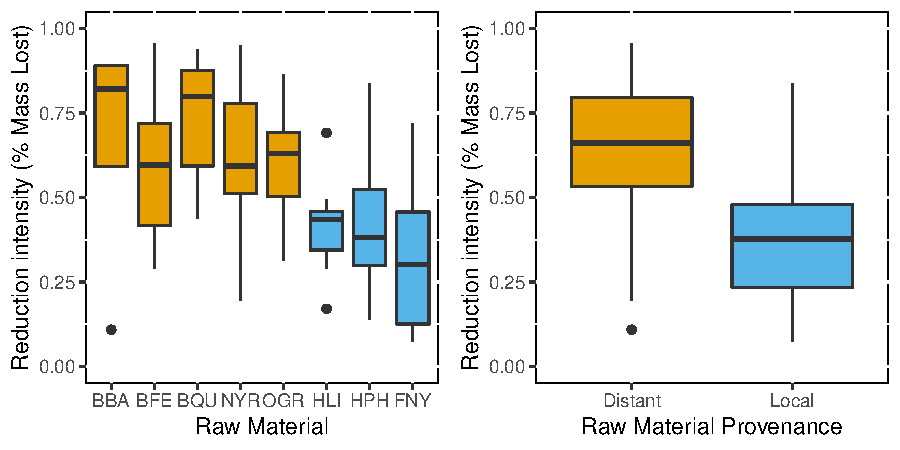
\includegraphics{HUMEV-D-20-00115_revised_draft_files/figure-latex/fig-3-1.pdf}
\caption{The distribution of core reduction intensity values as
predicted by the GLMM (Douglass et al 2018). The results show stark
differences in the degree of reduction in materials originating from
more distant sources than those that originate from local sources of
stone. \label{core_redux_rm}}
\end{figure}

This pattern of core utilization is also reflected in the flake
assemblages. Flake sequence values range from the first flakes off the
core to the 30th flake in the sequence. The largest differences are,
again, between rock types derived from more distant sources and those
found locally (Fig. \ref{flake_seq_rm}, Mann Whitney U, W=
\ensuremath{3.3325\times 10^{5}}, \emph{p} \textless{} .0001). Flakes
produced on rock types from more distant raw material sources are from
later in the reduction sequence, while flakes produced on raw materials
that are available locally are from earlier stages of reduction (Fig.
\ref{flake_seq_rm}). Interestingly, there is a striking amount of
homogeneity in the distribution of flake sequence values associated with
exotic or distant raw materials. With the exception of Bukoban Felsite
(BFe), the inter-quartile range of flake sequence values are very
similar from distant sources. Even though Bukoban Felsite has a wider
range than the other exotic materials, its median is quite similar. The
flake sequence values associated with the local materials are also
similar to each other but show slightly more variation.

\begin{figure}
\centering
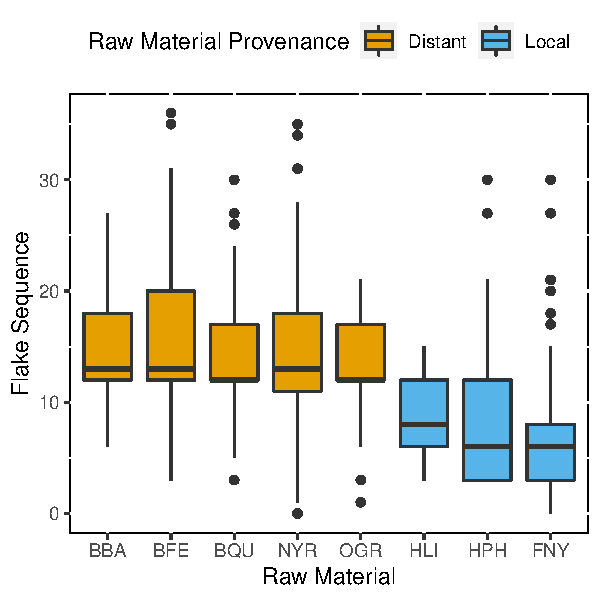
\includegraphics{HUMEV-D-20-00115_revised_draft_files/figure-latex/fig-4-1.pdf}
\caption{The distribution of flake sequence values present within the
Kanjera South flake assemblage. As is the case with the core assemblage,
the primary differences in flake sequence values are between materials
originating from more distant sources and those that originate from
local sources of stone. \label{flake_seq_rm}}
\end{figure}

As previously reported, the Kanjera core assemblage is comprised of a
wide variety of technological types and core reduction strategies (Braun
et al., 2009a). The frequency of core reduction strategies present has a
significant relationship with the raw material type (Fisher's exact
test, \emph{p} = \ensuremath{5\times 10^{-4}} ). Though unifacial and
unidirectional reduction strategies are present in small frequencies,
there is a greater representation of centripetal, bifacial and
multifacial exploitation strategies in materials from more distant
origins (Fig. \ref{core.tech}). On the other hand, local materials such
as the Fenetized Nyanzian (FNy) and Homa Phonolite (HPh) are represented
by greater number of unifacial or unidirectional core reduction
strategies (Fig. \ref{core.tech}). Contrary to this general pattern,
cores produced from some of the local materials {[}e.g.~Homa Limestone
(HLi){]} are often multifacially reduced. However, as addressed in the
discussion, this is likely related to the properties of the raw material
itself (Braun et al., 2009).When the core reduction intensity values for
each reduction strategy are considered, unifacial and unipolar cores are
reduced less than bifacial, multifacial or polyhedral cores (Kruskal
Wallis, chi-squared = 57.07, p \textless{} 0.0001) (Fig.
\ref{core.tech}). In other words, core reduction strategies that require
fewer core rotations, such as unifacial and unidirectional strategies,
are less reduced than those that that involved more complex patterns.

\begin{figure}
\centering
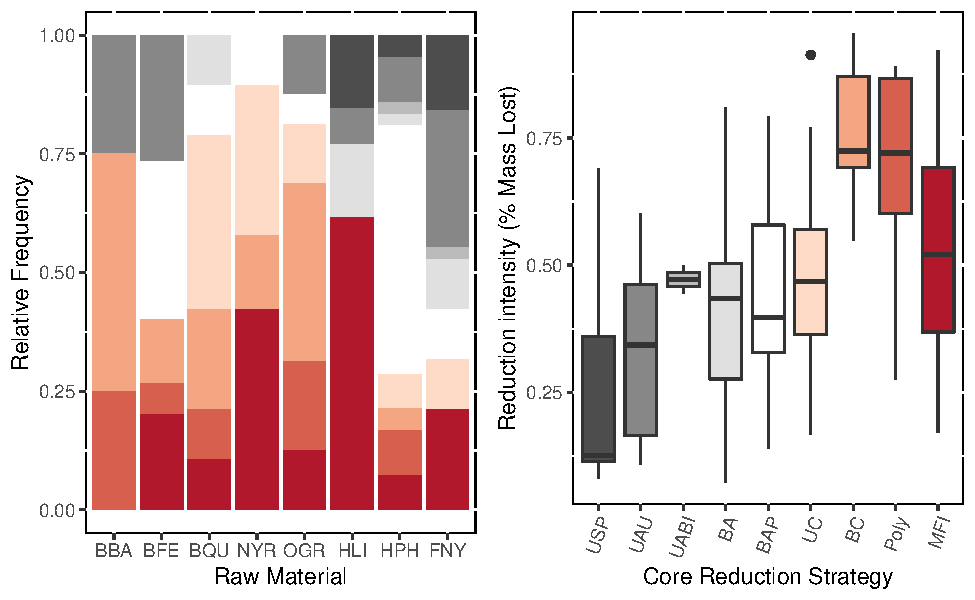
\includegraphics{HUMEV-D-20-00115_revised_draft_files/figure-latex/fig-5-1.pdf}
\caption{Left: The distribution of core reduction strategies by raw
material type. With the exception of Homa Limestone, raw materials that
derive from the Kisi highlands are more greatly represented by complex
core reduction strategies than those that can be found in the immediate
vicinity of Kanjera South. Right: The distribution of reduction
intensity values according to reduction strategy. \textbf{USP}:
Unifacial Simple Partial. \textbf{UAU}: Unidirectional abrupt unifacial.
\textbf{UABI}: Unifacial abrupt bidirectional. \textbf{BA}:
Bidirectional Abrupt. \textbf{BAP} Bifacial Partial. \textbf{UC}:
Unifacial centripetal. \textbf{BC}: Bifacial Centripetal. \textbf{Poly}:
Polyhedral. \textbf{MFI}: Mutifacial Irregular. The colors of the
boxplots correspond with the representation of different reduction
strategies in the left figure. \label{core.tech}}
\end{figure}

\hypertarget{flake-efficiency}{%
\subsection{3.2. Flake efficiency}\label{flake-efficiency}}

Analysis of the relative proportion of flake edge to mass indicates
significantly different technological strategies applied to the
different raw materials from the Kanjera South assemblage. Although the
mean values of raw materials are relatively similar, the overall
distribution indicates that rock types from sources that are further
away from Kanjera South (e.g.~NyR, BFe, BQu) are produced in a way that
allows for much higher efficiency values than those seen in the rock
types found close to Kanjera South (Mann-Whitney U, W=
\ensuremath{1.91209\times 10^{5}}, p \textless{} .0001). It should be
noted that even though there are significant differences between the
edge to mass ratios, the distributions show overlap (Fig.
\ref{flake_efficiency}). This indicates that it is physically possible
to produce flakes with similar edge to mass ratios in each raw material
type. Given the results of the core reduction intensity and flake
sequence analysis, it could also be argued that the observed differences
in flake efficiency could simply reflect the varying levels of reduction
intensity observed between the distant and local assemblage. However,
Fig. \ref{flake_efficiency} (right) suggests that there is no strong
relationship between flake sequence and flake efficiency. This suggests
that hominins at Kanjera South did not implement this strategy as
frequently on raw materials that were locally abundant. Hominins at
Kanjera South consistently produced flakes with greater edge and less
mass from rock types that came from more distant sources.

\begin{figure}
\centering
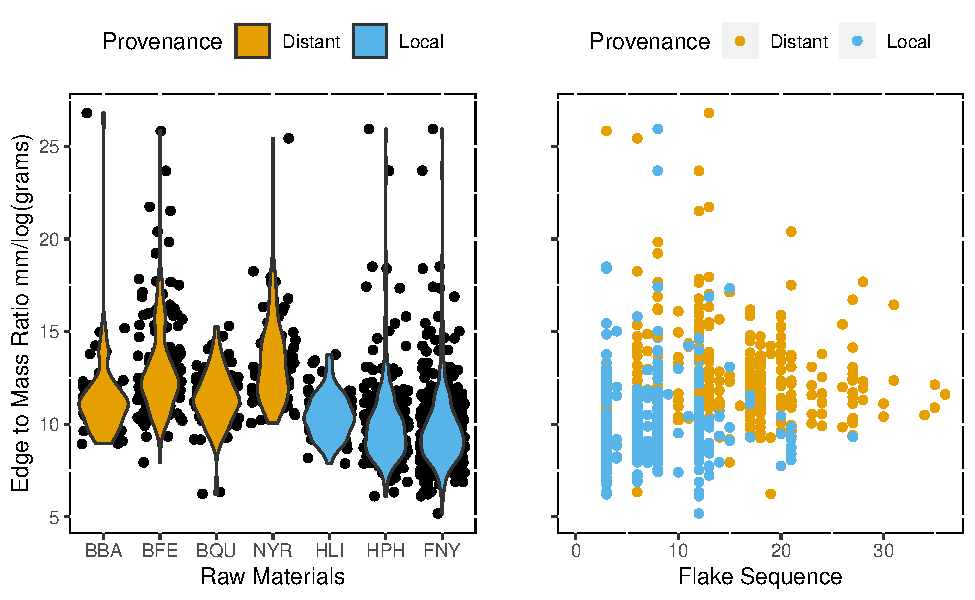
\includegraphics{HUMEV-D-20-00115_revised_draft_files/figure-latex/fig-6-1.pdf}
\caption{Left: Boxplots of the measures of flake efficiency. Y-axis
represents perimeter of flakes divided by a logarithmically transformed
mass value. Right: A scatter plot examining the relationship between
flake efficiency and flake sequence. \label{flake_efficiency}}
\end{figure}

\hypertarget{discussion}{%
\section{4. Discussion}\label{discussion}}

\hypertarget{inferring-land-use-at-kanjera-south}{%
\subsection{4.1 Inferring land-use at Kanjera
South}\label{inferring-land-use-at-kanjera-south}}

The results of this study show an interaction between stone tool
utilization, raw material type and core reduction strategies. The most
striking distinction is the difference in the degree of utilization of
materials from local and exotic sources. This is also reflected in the
flake sequence data. To some extent, this can be explained by the poor
quality of some of the local materials. As discussed in Braun et. al
(2009a), removal sequences in local fenetized rocks (FNy) tend to be
short because of the presence of preexisting internal fracture planes
present in the highly metasomatized rocks. The chalky nature and
block-like geometry of Homa limestone (HLi) also limits the number of
flakes that can be removed. In contrast, the majority of raw materials
from more distant sources possess fewer flaws and fracture more
predictably than those found locally (Braun et al., 2009a).

However, not all of the cores from local sources have internal flaws. In
particular, Homa phonolite does not have the defects common in the other
local raw materials but is still less reduced than the nonlocal raw
materials. The coarse-grained nature of Oyugis granite makes it
difficult to maintain angles of less than 90 degrees, thus limiting the
degree that the material could be reduced (Braun et al., 2009a). Despite
these limitations, Oyugis granite is still more reduced than any of the
local raw materials (Fig. \ref{flake_seq_rm}). The totality of these
data suggest that raw material properties play a role in reduction
intensity but do not explain all of the variation in the Kanjera South
assemblage.

These outstanding differences in the degree of stone utilization at
Kanjera South can be interpreted as the result of the continuous use of
the high quality exotic raw materials as they were moved across long
distances. The higher core reduction intensity values and greater flake
sequence values in the exotic material is consistent with a
distance-decay pattern of tool-use that has been documented in a variety
of time periods (Clark, 1979; Newman, 1994; Close, 1999; Blumenschine et
al., 2008; Luncz et al., 2016). Though this pattern has often been
associated with a high level of planning and foresight, modeling work
has demonstrated that differences in the reduction intensity of
materials from local and distant sources can arise simply due to
continuous transport even in the absence of a structured land-use
pattern {[}i.e., random movement, (Brantingham, 2003; Pop, 2016){]}.
However, the Kanjera South assemblage deviates from these neutral models
in one critical aspect. These models predict that the variance in tool
reduction intensity will also decrease with distance from the raw
material source (Brantingham, 2003, p.~501). In contrast with model
expectations, while exotic materials are reduced more substantially than
local materials, the interquartile ranges of flake sequence and core
reduction measures of assemblages from distant sources are as wide (or
wider) than those associated with local sources.

Therefore, the Kanjera South assemblage does not fit expectations under
neutral conditions. It has been hypothesized that such deviations from
the neutral model of this nature may arise due to increasingly linear
movements toward specific locations (Brantingham, 2003, 2006;
Blumenschine et al., 2008; Braun et al., 2008b). Moreover, subsequent
work modeling the influence of directed movement towards attractors has
shown that while a distance-decay pattern remains visible, tools from
earlier stages of reduction will be over-represented (i.e.~greater
variance in reduction, (Reeves, 2019). Thus, the greater than expected
range in variance in the reduction intensity of distantly sourced cores
may suggest that hominins directed their movement to Kanjera South. This
is not to say that hominins carried rocks directly to Kanjera South.
However, Kanjera South may have acted as an attractor on the Pleistocene
landscape where hominins frequently visited to carry out stone
tool-using behaviors. This supported by the fact that the lithics
included in this study were excavated from a 3-meter sequence suggesting
that the patterns evinced by this study are the result of the repeated
visitation by hominins over hundreds to thousands of years.

This attractiveness of Kanjera South is also supported by other
archaeological and paleoecological evidence. Numerous taphonomic studies
of the faunal assemblage from Kanjera South have verified that hominins
efficiently exploited small bovids and may have processed larger
carcasses that were scavenged from carnivores (Ferraro et al., 2013;
Oliver et al., 2019). Use-wear studies demonstrate that hominins carried
out a variety of resource processing activities with stone artifacts at
Kanjera South, including butchery and the processing of a variety of
plants, including underground storage organs (Lemorini et al., 2014,
2019). These studies suggest that hominins spent a great deal of time
producing stone tools for a variety of tasks. While the notion that
hominins directed their movement toward specific localities or ecotones
has been suggested at other localities (e.g.~Blumenschine et al., 2008,
2012a, 2012b), Kanjera South represents the earliest documented evidence
of this pattern. This reinforces that notion that Oldowan stone
tool-using behavior was strongly integrated into broader foraging
strategies of Early Pleistocene hominins. It may be that this pattern of
behavior, as has been suggested by Potts (1992), is synonymous with the
appearance of the Oldowan. This could be tested by future landscape
scale studies at the earliest localities such as Ledi Geraru and Gona
(Stout et al., 2010; Braun et al., 2019).

The land-use pattern elucidated at Kanjera South also differs from
younger Oldowan sites in scale. The movement pattern described at Koobi
Fora (Braun et al., 2008b) suggests that hominins directed their
movements across paleogeographic settings at a scale of hundreds of
meters. At Olduvai Gorge, the directed movement toward riparian
woodlands is thought to have occurred over a scale no greater than 5
kilometers (Blumenschine et al., 2008, 2012a). The data presented here
imply that a pattern of directed movement occurs at a scale of at least
10-13 kilometers for non-local materials. This is an interesting
distinction because Kanjera South is one of the few sites from this time
frame situated in an open grassland (Plummer et al., 2009b). Modern
humans tend to travel farther and more frequently in open arid
environments than those that live in more closed habitats (Kelly, 2007;
Burnside et al., 2012). Savanna-adapted chimpanzees from Fongoli,
Senegal also possess a larger home range and practice fission-fusion
less frequently (Pruetz and Bertolani, 2009). In this respect, the
increased scale of this structured land-use pattern at Kanjera South may
further attest to the adaptive flexibility of Oldowan hominins open
environments.

\hypertarget{the-influence-of-land-use-on-oldowan-production-strategies}{%
\subsection{4.2 The influence of land-use on Oldowan production
strategies}\label{the-influence-of-land-use-on-oldowan-production-strategies}}

The results of this study also suggest that patterns of land-use
influence the technical decisions of Oldowan tool makers. At Kanjera
South, exotic raw materials show a strong bias toward more reduced,
complete bifacial and multifacial reduction strategies, as opposed to
the more even representation of core reduction strategies among local
materials. This suggests that the broader pattern of stone tool
transport influenced the ways in which Oldowan hominins economized
stone. The relatively long transport distance, in combination with the
lower quality of material available near Kanjera South, may have
incentivized the retention of exotic raw materials in areas where
lithologies of such quality were less abundant. In this light, the high
frequency of bifacial and multifacial reduction strategies and the
higher cutting edge to mass ratios present in the exotic raw materials
may reflect a general need to maximize the utility that could be
extracted from these cores. The exploitation of multiple flake removal
surfaces allows a core to remain active in a toolkit for a longer period
of time.

In contrast, the predominantly unifacial and partial bifacial reduction
strategies in combination with the significantly lower edge to mass
ratio values may reflect a more expedient treatment of the lower quality
local raw materials. However, it must also be noted that some of the
technical variation within the local assemblage likely reflects the
constraints imposed by the quality of the raw material. The predominance
of irregular multi-facial strategies in the Homa limestone core
assemblage (HLi) is argued to be result of its chalky nature and
block-like geometry (Braun et al., 2009a). Therefore, this corpus of
information may indicate that Oldowan hominins where able to adopt
different technical strategies in order to mitigate the changing
qualities in available raw materials over large transport distances.
This pattern of exploitation, in the context of the broader land-use
strategy at Kanjera South, provides additional evidence for a high level
of planning and foresight in Oldowan hominins.

These results also have broader implications for how techno-economic
variation arises in the Oldowan record. The variability in the Oldowan
record is often interpreted through a socio-cognitive lens, in which
technological differences between assemblages are argued to reflect
socially learned information that particularize various groups or
individuals (Delagnes and Roche, 2005; Roche et al., 2009, 2018; Stout,
2011; Stout et al., 2019). More recently, these criteria have been used
to argue for the presence of copying social learning mechanisms in the
earliest Oldowan (Stout et al., 2019). However, the results of this
study strongly link the application of various technical strategies with
the broader land-use system in which tool-use is incorporated. Moreover,
the fact that core reduction intensity seems to increase as cores are
increasingly rotated further suggests that unifacial, bifacial and
multifacial cores may not reflect discrete strategies but are rather
points on continuum of reduction that arise out of a need to maximize
the utility of high-quality materials.

The notion that Oldowan stone tool variation may reflect a continuum of
utilization has been previously suggested based on evidence from
controlled least effort experiments by Toth (1982) and later by Moore
and Perston (2016). Potts (1991) suggested that this also may be the
case with cores at Olduvai Gorge by showing how different core types
varied according to mass. By directly estimating the amount of mass lost
from each core in the assemblage, we find further support for this
notion as the various core exploitation strategies present at Kanjera
South are correlated with reduction intensity. In light of the results
of this study, the frequent use of unifacial reduction strategies at
sites such as Lokalelei 2C, East Gona, Hadar, Omo, Ledi Geraru may
relate to the overall abundance of knappable material that is
immediately available at these sites (Kimbel et al., 1996; Roche et al.,
1999; Stout et al., 2005; Braun et al., 2019)

Finally, while the preceding analysis emphasizes the role of the broader
environment and land-use on technological variability, ecology is not
the sole driver of Oldowan technical variation. The inter-quartile
ranges in Fig. \ref{flake_efficiency} show a substantial amount of
overlap between the reduction intensity and core reduction strategies.
This suggests that not all variation can be explained by environmental
parameters such as raw material availability and material properties.
Moreover, at other localities (e.g.~West Turkana) inter-site differences
are not easily explained by factors such as raw material availability
alone (Roche et al., 2018). This unexplained variation may be the result
of socio-cultural dynamics that may have maintained information
regarding the stone tool production process between groups. However, the
fidelity and the mechanisms that underlie the maintenance of this
information remain an open debate (Hovers, 2012; Morgan et al., 2015;
Tennie et al., 2016, 2017; Stout et al., 2019). Nevertheless, the
application of quantitative measures of core reduction intensity, flake
sequence, and edge to mass ratio, in combination with broader contextual
information regarding raw material quality and provenance, further
elucidate the relationship between hominin land-use and Oldowan
technical decision making.

\hypertarget{conclusion}{%
\section{5.0 Conclusion}\label{conclusion}}

Despite the superficial simplicity of the Oldowan, its variability
reflects a complex interaction of ecological, behavioral and social
factors. The combination of quantitative measures of stone tool
reduction with qualitative characterizations of lithic technology
(e.g.~Braun et al., 2009; Plummer and Bishop, 2016) provides new
insights into the ecological factors that influence Oldowan technology,
and hominin behavior. At Kanjera South, exotic materials are more
substantially reduced than local materials, reflecting differences in
the quality of the lithologies available. The durability and hardness of
exotic materials (Braun et al., 2009a) would have incentivized their
transport over longer distances (Braun et al., 2008a). Differences in
reduction highlight that Oldowan tools were part of a mobile tool kit
that reflects a broader land-use strategy. The marked differences in
reduction intensity in combination with the paucity of early sequence
flakes suggest that exotic materials were often utilized prior to their
arrival at Kanjera South. Although exotic materials are more reduced
than local materials, the variance in the amount of stone tool reduction
does not adhere to neutral expectations. This result suggests that the
lithic assemblage at Kanjera South reflects a structured land-use
pattern where hominins may have directed their movement, at least on
occasion, to Kanjera South.

This pattern also appears to have an influence on the technological
strategies employed by Oldowan tool makers at Kanjera South. The
relationship between core reduction strategies and reduction intensity
indicates that raw material quality and provenance have a strong
influence on the technological variation observed within a lithic
assemblage. While these results show that ecological parameters have a
strong effect on stone tool variation, a substantial amount of variation
remains unexplained by ecology alone. Future studies should utilize an
integrated approach to understand the behavioral significance of the
Oldowan.

\hypertarget{supplementary-material}{%
\section{Supplementary Material:}\label{supplementary-material}}

S1: A link to where the data underlying this analysis and the R code
used to conduct the analysis can be downloaded and viewed.
\href{https://www.dropbox.com/home/Models_and_Runs/Kanjera\%20South}{Link}.

\hypertarget{acknowledgements}{%
\section{Acknowledgements}\label{acknowledgements}}

We thank the National Museums of Kenya and M. Kibunjia, F.K. Manthi, R.
Kinyanjui, J. Kibii and E. Ndiema for support. J.M. Nume and B. Onyango
managed the Kanjera field teams. We acknowledge Kenya Government
permission granted by the Ministry of Sports, Culture and the Arts, and
by NACOSTI permit P/14/7709/701. Funding from the L.S.B. Leakey
Foundation, the National Geographic Society, the National Science
Foundation, the Wenner--Gren Foundation and the Professional Staff
Congress--City University of New York Research Award Program to TP for
Kanjera field and laboratory work is gratefully acknowledged. We would
like to thank Rick Potts and the Human Origins Program at the
Smithsonian Institution for support during all phases of the Kanjera
research, and the Peter Buck Fund for Human Origins Research.

\hypertarget{references}{%
\section{References}\label{references}}

Behrensmeyer, A.K., Potts, R., Plummer, T.W., Tauxe, L., Opdyke, N.,
Jorstad, T., 1995. The Pleistocene locality of Kanjera, Western Kenya:
stratigraphy, chronology and paleoenvironments. Journal of Human
Evolution. 29, 247--274.

Blumenschine, R.J., Masao, F.T., Stollhofen, H., Stanistreet, I.G.,
Bamford, M.K., Albert, R.M., Njau, J.K., Prassack, K.A., 2012a.
Landscape distribution of Oldowan stone artifact assemblages across the
fault compartments of the eastern Olduvai Lake Basin during early
lowermost Bed II times. Journal of Human Evolution. 63, 384--394.

Blumenschine, R.J., Masao, F.T., Tactikos, J.C., Ebert, J.I., 2008.
Effects of distance from stone source on landscape-scale variation in
Oldowan artifact assemblages in the Paleo-Olduvai Basin, Tanzania.
Journal of Archaeological Science. 35, 76--86.

Blumenschine, R.J., Peters, C.R., 1998. Archaeological predictions for
hominid land use in the paleo-Olduvai Basin, Tanzania, during lowermost
Bed II times. Journal of Human Evolution. 34, 565--607.

Blumenschine, R.J., Stanistreet, I.G., Njau, J.K., Bamford, M.K., Masao,
F.T., Albert, R.M., Stollhofen, H., Andrews, P., Prassack, K.A.,
McHenry, L.J., Fernández-Jalvo, Y., Camilli, E.L., Ebert, J.I., 2012b.
Environments and hominin activities across the FLK Peninsula during
Zinjanthropus times (1.84 Ma), Olduvai Gorge, Tanzania. Journal of Human
Evolution. 63, 364--383.

Brantingham, P.J., 2003. A Neutral Model of Stone Raw Material
Procurement. American Antiquity. 68, 487--509. Brantingham, P.J., 2006.
Measuring Forager Mobility. Current Anthropology. 47, 435--459.

Braun, D.R., Aldeias, V., Archer, W., Arrowsmith, J.R., Baraki, N.,
Campisano, C.J., Deino, A.L., DiMaggio, E.N., Dupont-Nivet, G., Engda,
B., Feary, D.A., Garello, D.I., Kerfelew, Z., McPherron, S.P.,
Patterson, D.B., Reeves, J.S., Thompson, J.C., Reed, K.E., 2019.
Earliest known Oldowan artifacts at \textgreater{}2.58 Ma from
Ledi-Geraru, Ethiopia, highlight early technological diversity.
Proceedings of the National Academy of Sciences. 116, 11712--11717.

Braun, D.R., Harris, J.W.K., 2003. Technological Developments in the
Oldowan of Koobi Fora: Innovative Techniques of Artifact Analysis.
p.~29.

Braun, D.R., Plummer, T., Ditchfield, P., Ferraro, J.V., Maina, D.,
Bishop, L.C., Potts, R., 2008a. Oldowan behavior and raw material
transport: perspectives from the Kanjera Formation. Journal of
Archaeological Science. 35, 2329--2345.

Braun, D.R., Plummer, T.W., Ditchfield, P.W., Bishop, L.C., Ferraro,
J.V., 2009a. Oldowan Technology and Raw Material Variability at Kanjera
South. In: Interdisciplinary Approaches to the Oldowan, Vertebrate
Paleobiology and Paleoanthropology. Springer Netherlands, Dordrecht,
pp.~99--110.

Braun, D.R., Plummer, T.W., Ferraro, J.V., Ditchfield, P., Bishop, L.C.,
2009b. Raw material quality and Oldowan hominin toolstone preferences:
evidence from Kanjera South, Kenya. Journal of Archaeological Science.
36, 1605--1614.

Braun, D.R., Rogers, M.J., Harris, J.W.K., Walker, S.J., 2008b.
Landscape-scale variation in hominin tool use: Evidence from the
Developed Oldowan. Journal of Human Evolution. 55, 1053--1063.

Braun, D.R., Tactikos, J.C., Ferraro, J.V., Arnow, S.L., Harris, J.W.K.,
2008c. Oldowan reduction sequences: methodological considerations.
Journal of Archaeological Science. 35, 2153--2163.

Braun, D.R., Tactikos, J.C., Ferraro, J.V., Harris, J.W.K., 2005. Flake
recovery rates and inferences of Oldowan hominin behavior: a response
to. Journal of Human Evolution. 48, 525--531.

Burnside, W.R., Brown, J.H., Burger, O., Hamilton, M.J., Moses, M.,
Bettencourt, L.M.A., 2012. Human macroecology: Linking pattern and
process in big-picture human ecology. Biological Reviews. 87, 194--208.

Clark, J.R., 1979. Measuring the Flow of Goods with Archaeological Data.
Economic Geography. 55, 1.

Clarkson, C., 2013. Measuring core reduction using 3D flake scar
density: a test case of changing core reduction at Klasies River Mouth,
South Africa. Journal of Archaeological Science. 40, 4348--4357.

Close, A.E., 1999. Distance and decay: an uneasy relationship.
Antiquity. 73, 24--32.

Cotterell, B., Kamminga, J., Dickson, F.P., 1985. The essential
mechanics of conchoidal flaking. International Journal of Fracture. 29,
205--221.

de la Torre, I., 2004. Omo Revisited: Evaluating the Technological
Skills of Pliocene Hominids. Current Anthropology. 45, 439--465.

de la Torre, I., Mora, R., 2005. Technological Strategies in the Lower
Pleistocene at Olduvai Beds I and II. Service de Prehistoire, Universite
de Liege, Liege.

de la Torre Ignacio, I., 2011. The Early Stone Age lithic assemblages of
Gadeb (Ethiopia) and the Developed Oldowan/early Acheulean in East
Africa. Journal of Human Evolution. 60, 768--812.

de Torre, I. la, Mora, R., 2009. Remarks on the Current Theoretical and
Methodological Approaches to the Study of Early Technological Strategies
in Eastern Africa. In: Hovers, E., Braun, D.R. (Eds.), Interdisciplinary
Approaches to the Oldowan, Vertebrate Paleobiology and
Paleoanthropology. Springer Netherlands, Dordrecht, pp.~15--24.

Delagnes, A., Roche, H., 2005. Late Pliocene hominid knapping skills:
The case of Lokalalei 2C, West Turkana, Kenya. Journal of Human
Evolution. 48, 435--472.

Ditchfield, P.W., Whitfield, E., Vincent, T., Plummer, T., Braun, D.,
Deino, A., Hertel, F., Oliver, J.S., Louys, J., Bishop, L.C., 2019.
Geochronology and physical context of Oldowan site formation at Kanjera
South, Kenya. Geological Magazine. 156, 1190--1200.

Douglass, M.J., Lin, S.C., Braun, D.R., Plummer, T.W., 2018. Core
Use-Life Distributions in Lithic Assemblages as a Means for
Reconstructing Behavioral Patterns. Journal of Archaeological Method and
Theory. 1--35.

Ferraro, J.V., Plummer, T.W., Pobiner, B.L., Oliver, J.S., Bishop, L.C.,
Braun, D.R., Ditchfield, P.W., Iii, J.W.S., Binetti, K.M., Jr, J.W.S.,
Hertel, F., Potts, R., 2013. Earliest Archaeological Evidence of
Persistent Hominin Carnivory. PLOS ONE. 8, e62174.

Finestone, E.M., Braun, D.R., Plummer, T.W., Bartilol, S., Kiprono, N.,
2020. Building ED-XRF datasets for sourcing rhyolite and quartzite
artifacts: A case study on the Homa Peninsula, Kenya. Journal of
Archaeological Science: Reports. 33, 102510.

Gallotti, R., 2018. Before the Acheulean in East Africa: An Overview of
the Oldowan Lithic Assemblages. In: Gallotti, R., Mussi, M. (Eds.), The
Emergence of the Acheulean in East Africa and Beyond. Springer
International Publishing, Cham, pp.~13--32.

Goldman-Neuman, T., Hovers, E., 2012. Raw material selectivity in Late
Pliocene Oldowan sites in the Makaamitalu Basin, Hadar, Ethiopia.
Journal of Human Evolution. 62, 353--366.

Gotelli, N.J., Ellison, A.M., 2013. A primer of ecological statistics,
Second edition. ed. Sinauer Associates, Inc., Publishers, Sunderland,
Massachusetts.

Hay, R.L., 1976. Geology of the Olduvai Gorge. University of California
Press, Los Angeles.

Hovers, E., 2009. Learning From Mistakes: Flaking Accidents and Knapping
Skills in the Assemblage of A.L. 894 (Hadar, Ethiopia). In: Schick,
K.D., Toth, N. (Eds.), The Cutting Edge: New Apporaches to the
Archaeology of Human Origins. Stone Age Institute, Gosport, IN,
pp.~137--139.

Hovers, E., 2012. Invention, Reinvention and Innovation. In:
Developments in Quaternary Sciences. Elsevier, pp.~51--68.

Isaac, G., 1984. The archaeology of human origins: Studies of the Lower
Pleistocene in East Africa, 1971-1981. In: Advances in World
Archaeology. pp.~1--86.

Isaac, G.Ll., 1981. Stone Age visiting cards: approaches to the study of
early land use patterns. In: Pattern of the Past: Studies in Honour of
David Clarke. University of Cambridge Press, Cambridge, pp.~131--155.

Isaac, G.Ll., Harris, J.W.K., 1976. The Scatter Between the Patches. In:
The Krober Anthropological Society. Unpublished, Berkeley.

Kelly, R.L., 2007. The Foraging Spectrum: Diversity in Hunter-Gatherer
Lifeways, Reprint edition. ed. Percheron Press/Eliot Werner
Publications, Clinton Corners, New York.

Kimbel, W.H., Walter, R.C., Johanson, D.C., Reed, K.E., Aronson, J.L.,
Assefa, Z., Marean, C.W., Eck, G.G., Bobe, R., Hovers, E., Rak, Y.,
Vondra, C., Yemane, T., York, D., Chen, Y., Evensen, N.M., Smith, P.E.,
1996. Late Pliocene Homo and Oldowan Tools from the Hadar Formation
(Kada Hadar Member), Ethiopia. Journal of Human Evolution. 31, 549--561.

Kuhn, S.L., 1990. A geometric index of reduction for unifacial stone
tools. Journal of Archaeological Science. 17, 583--593.

Le Bas, M.J., 1977. Carbonatite-Nephelinite Volcanism: An African Case
History. Cambridge University Press, Cambridge.

Lemorini, C., Bishop, L.C., Plummer, T.W., Braun, D.R., Ditchfield,
P.W., Oliver, J.S., 2019. Old stones' song---second verse: use-wear
analysis of rhyolite and fenetized andesite artifacts from the Oldowan
lithic industry of Kanjera South, Kenya. Archaeological and
Anthropological Sciences. 11, 4729--4754.

Lemorini, C., Plummer, T.W., Braun, D.R., Crittenden, A.N., Ditchfield,
P.W., Bishop, L.C., Hertel, F., Oliver, J.S., Marlowe, F.W.,
Schoeninger, M.J., Potts, R., 2014. Old stones' song: Use-wear
experiments and analysis of the Oldowan quartz and quartzite assemblage
from Kanjera South (Kenya). Journal of Human Evolution. 72, 10--25.

Li, H., Kuman, K., Li, C., 2015. Quantifying the Reduction Intensity of
Handaxes with 3D Technology: A Pilot Study on Handaxes in the
Danjiangkou Reservoir Region, Central China. PLOS ONE. 10, e0135613.

Lombao, D., Cueva-Temprana, A., Rabuñal, J.R., Morales, J.I., Mosquera,
M., 2019. The effects of blank size and knapping strategy on the
estimation of core's reduction intensity. Archaeological and
Anthropological Sciences. 11, 5445--5461.

Luncz, L.V., Proffitt, T., Kulik, L., Haslam, M., Wittig, R.M., 2016.
Distance-decay effect in stone tool transport by wild chimpanzees.
Proceedings of the Royal Society B: Biological Sciences. 283, 20161607.

Moore, M.W., Perston, Y., 2016. Experimental Insights into the Cognitive
Significance of Early Stone Tools. PLOS ONE. 11, e0158803.

Morgan, T.J.H., Uomini, N.T., Rendell, L.E., Chouinard-Thuly, L.,
Street, S.E., Lewis, H.M., Cross, C.P., Evans, C., Kearney, R., Torre,
I. de la, Whiten, A., Laland, K.N., 2015. Experimental evidence for the
co-evolution of hominin tool-making teaching and language. Nature
Communications. 6, 1--8.

Newman, J.R., 1994. The Effects of Distance on Lithic Material Reduction
Technology. Journal of Field Archaeology. 21, 491--501.

Oliver, J.S., Plummer, T.W., Hertel, F., Bishop, L.C., 2019. Bovid
mortality patterns from Kanjera South, Homa Peninsula, Kenya and
FLK-Zinj, Olduvai Gorge, Tanzania: Evidence for habitat mediated
variability in Oldowan hominin hunting and scavenging behavior. Journal
of Human Evolution. 131, 61--75.

Plummer, T.W., 2004. Flaked stones and old bones: Biological and
cultural evolution at the dawn of technology. Yearbook of Physical
Anthropology. 47, 118--164.

Plummer, T.W., Bishop, L.C., Ditchfield, P.W., Ferraro, J.V., Kingston,
J.D., Hertel, F., Braun, D.R., 2009a. The Environmental Context of
Oldowan Hominin Activities at Kanjera South, Kenya. In: Hovers, E.,
Braun, D.R. (Eds.), Interdisciplinary Approaches to the Oldowan,
Vertebrate Paleobiology and Paleoanthropology. Springer Netherlands,
Dordrecht, pp.~149--160.

Plummer, T.W., Bishop, L.C., Ditchfield, P.W., Hicks, J., 1999. Research
on Late Pliocene Oldowan Sites at Kanjera South, Kenya. Journal of Human
Evolution. 36, 151--170.

Plummer, T.W., Ditchfield, P.W., Bishop, L.C., Kingston, J.D., Ferraro,
J.V., Braun, D.R., Hertel, F., Potts, R., 2009b. Oldest evidence of
toolmaking hominins in a grassland-dominated ecosystem. PLoS ONE. 4.

Pop, C.M., 2016. Simulating Lithic Raw Material Variability in
Archaeological Contexts: A Re-evaluation and Revision of Brantingham's
Neutral Model. Journal of Archaeological Method and Theory. 23,
1127--1161.

Potts, R., 1988. Early Hominid Activities at Olduvai: Foundations of
Human Behaviour. Aldine de Gruyter, New York.

Potts, R., 1991. Why the Oldowan? Plio-Pleistocene Toolmaking and the
Transport of Resources. Journal of Anthropological Research. 47,
153--176.

Potts, R., 1994. Variables versus models of early Pleistocene hominid
land use. Journal of Human Evolution. 27, 7--24.

Potts, R., Behrensmeyer, A.K., Ditchfield, P., 1999. Paleolandscape
variation and early Pleistocene hominid activities: Members 1 and 7,
Olorgesailie formation, Kenya. Journal of Human Evolution. 37, 747--788.

Pruetz, J., Bertolani, P., 2009. Chimpanzee (Pan troglodytes verus)
Behavioral Responses to Stresses Associated with Living in a
Savannah-Mosaic Environment: Implications for Hominin Adaptations to
Open Habitats. PaleoAnthropology. 2009, 252--262. Reeves, J.S., 2019.
Digital Stone Age Visiting Cards: Quantitative approaches to Early
Pleistocene hominin land use (PhD Thesis). George Washington University,
Washington D.C.

Roche, H., Blumenschine, R.J., Shea, J.J., 2009. Origins and Adaptations
of Early Homo: What Archeology Tells Us. In: Grine, F.E., Fleagle, J.G.,
Leakey, R.E. (Eds.), The First Humans -- Origin and Early Evolution of
the Genus Homo. Springer Netherlands, Dordrecht, pp.~135--147.

Roche, H., de la Torre, I., Arroyo, A., Brugal, J.-P., Harmand, S.,
2018. Naiyena Engol 2 (West Turkana, Kenya): a Case Study on Variability
in the Oldowan. African Archaeological Review. 35, 57--85.

Roche, H., Delagnes, A., Brugal, J.-P., Feibel, C., Kibunjia, M.,
Mourre, V., Texier, P.-J., 1999. Early hominid stone tool production and
technical skill 2.34 Myr ago in West Turkana, Kenya. Nature. 399,
57--60.

Saggerson, E.P., 1952. Geology of the Kisumu District. Geological Survey
of Kenya, Republic of Kenya, Mines and Geological Department,.

Schick, K.D., 1987. Modeling the formation of Early Stone Age artifact
concentrations. Journal of Human Evolution. 16, 789--807.

Schick, K.D., Toth, N.P., 1994. Making silent stones speak: Human
evolution and the dawn of technology. Simon and Schuster.

Schick, K.D., Toth, N.P., Stone Age Institute (Eds.), 2006. An Overview
of the Oldowan Industrial Complex: The sites and the nature of their
evidence. In: The Oldowan: Case Studies into the Earliest Stone Age,
Stone Age Institute Publication Series. Stone Age Institute, Gosport,
IN, pp.~1--42.

Semaw, S., 2000. The World's Oldest Stone Artefacts from Gona, Ethiopia:
Their Implications for Understanding Stone Technology and Patterns of
Human Evolution Between 2·6--1·5 Million Years Ago. Journal of
Archaeological Science. 27, 1197--1214.

Stout, D., 2011. Stone toolmaking and the evolution of human culture and
cognition. Philosophical Transactions of the Royal Society B: Biological
Sciences. 366, 1050--1059.

Stout, D., Chaminade, T., 2009. Making tools and making sense: Complex,
intentional behaviour in human evolution. Cambridge Archaeological
Journal. 19, 85--96.

Stout, D., Quade, J., Semaw, S., Rogers, M.J., Levin, N.E., 2005. Raw
material selectivity of the earliest stone toolmakers at Gona, Afar,
Ethiopia. Journal of Human Evolution. 48, 365--380.

Stout, D., Rogers, M.J., Jaeggi, A.V., Semaw, S., 2019. Archaeology and
the Origins of Human Cumulative Culture: A Case Study from the Earliest
Oldowan at Gona, Ethiopia. Current anthropology: A world journal of the
sciences of man. 309--340.

Stout, D., Semaw, S., Rogers, M.J., Cauche, D., 2010. Technological
variation in the earliest Oldowan from Gona, Afar, Ethiopia. Journal of
Human Evolution. 58, 474--491.

Tennie, C., Braun, D.R., Premo, L.S., McPherron, S.P., 2016. The Island
Test for Cumulative Culture in the Paleolithic. In: Haidle, M.N.,
Conard, N.J., Bolus, M. (Eds.), The Nature of Culture. Springer
Netherlands, Dordrecht, pp.~121--133.

Tennie, C., Premo, L.S., Braun, D.R., McPherron, S.P., 2017. Early Stone
Tools and Cultural Transmission: Resetting the Null Hypothesis. Current
Anthropology. 58, 000--000.

Toth, N., 1982. The Stone Technologies of Early Hominids at Koobi Fora,
Kenya: An Experimental Approach (Doctoral Dissertation). Univversity of
California, Berkeley.

Toth, N., 1985. The oldowan reassessed: A close look at early stone
artifacts. Journal of Archaeological Science. 12, 101--120.

Toth, N., 1987. Behavioral inferences from Early Stone artifact
assemblages: an experimental model. Journal of Human Evolution. 16,
763--787.

Toth, N., Schick, K., 2018. An overview of the cognitive implications of
the Oldowan Industrial Complex. Azania: Archaeological Research in
Africa. 53, 3--39.


\end{document}


